\chapter{Các kết quả thí nghiệm}
\label{Chapter4}

% \noindent\textit{Trong chương này, nhóm chúng em trình bày các kết quả thí nghiệm để đánh giá các đề xuất tìm hiểu được từ bài báo đã được nói ở chương trước. Bộ dữ liệu được dùng để tiến hành thí nghiệm là bộ COAT (bao gồm đánh giá của người dùng cho áo khoác), bộ Yahoo (bao gồm đánh giá của người dùng cho các bài hát), bộ Movielens 100K (bao gồm đánh giá của người dùng cho các bộ phim). Các kết quả thí nghiệm cho thấy khi khi dùng IPS đánh giá mô hình hoàn toàn khớp với hiệu suất thật và tốt hơn nhiều so với các độ đo đánh giá truyền thống. Các kết quả thí nghiệm cũng cho thấy mô hình được huấn luyện dựa trên độ đo IPS cũng cho kết quả tổng quát hóa tốt hơn trên các mức độ selection bias khác nhau.}

\section{Các thiết lập thí nghiệm}
\label{sec:4_setup}
\subsection{Các tập dữ liệu}
Nhóm chúng em sẽ tiến hành các thí nghiệm về hiệu năng của mô hình ``Matrix factorization'' truyền thống (MF) so với ``Matrix factorization'' sử dụng độ đo IPS (MF-IPS). Các thí nghiệm về hiệu năng này sẽ được đánh giá trên 2 tập dữ liệu Coat Shopping và Yahoo!R3, 2 tập dữ liệu này đều có tập training bị thiên lệch dữ liệu do người dùng tự lựa chọn chọn sản phẩm để đánh giá; và có một tập test không bị thiên lệch do người dùng đánh giá một tập các sản phẩm ngẫu nhiên. Thông tin cụ thể của từng tập dữ liệu được mô tả như sau:
\begin{itemize}
    \item Tập dữ liệu Coat Shopping: tập dữ liệu này chứa đánh giá của các người dùng cho các áo khoác, được thu thập bằng cách mô phỏng dữ liệu bị thiên lệch của những người dùng mua áo khoác trong cửa hàng trực tuyến. Những người dùng được yêu cầu phải đánh giá 24 chiếc áo khoác họ tự chọn và 16 chiếc áo khoác được chọn ngẫu nhiên theo phân phối đều dựa trên thang điểm từ 1 đến 5. Tập dữ liệu chứa đánh giá từ 290 người dùng cho 300 sản phẩm. Các điểm đánh giá do người dùng tự lựa chọn sẽ được sử dụng làm tập huấn luyện, đồng thời, các điểm đánh giá trên tập các sản phẩm ngẫu nhiên sẽ được dùng để kiểm tra. 
    \item Tập dữ liệu Yahoo!R3: tập dữ liệu này chứa đánh giá của các người dùng cho các bài hát. Tập dữ liệu huấn luyện bị thiên lệch cung cấp hơn 300 nghìn đánh giá cho các bài hát, các bài hát này được tự lựa chọn bởi 15400 người dùng. Tập dữ liệu kiểm tra chứa đánh giá của 5400 người dùng cho 10 bài hát được chọn ngẫu nhiên theo phân phối đều.
\end{itemize}

Ngoài ra, nhằm đánh giá ảnh hưởng của việc dữ liệu bị thiên lệch tới việc học của MF và MF-IPS nhóm chúng em còn tiến hành thí nghiệm trên tập dữ liệu MovieLens 100k. Tập dữ liệu này chứa đánh giá của các người dùng cho các bộ phim. Tập dữ liệu MovieLens 100k sẽ chứa 100 000 đánh giá (từ 1 đến 5) của 943 người dùng trên 1682 bộ phim, trong đó mỗi người dùng sẽ đánh giá ít nhất 20 bộ phim. Các bộ phim được đánh giá trong tập dữ liệu này đều do người dùng tự lựa chọn, vì vậy đây là một tập dữ liệu bị thiên lệch. Do đó để thí nghiệm về ảnh hưởng của dữ liệu bị thiên lệch nhóm chúng em sẽ tiến hành tạo một bộ dữ liệu MovieLens 100k giả lập dựa trên bộ dữ liệu gốc, cách tạo bộ dữ liệu giả lập này sẽ được nhóm chúng em giới thiệu cụ thể trong phần \ref{subsection:MovieLens}.

\subsection{Các thiết lập về huấn luyện và kiểm tra}
Trong tất cả các thí nghiệm, nhóm chúng em sẽ tiến hành lựa chọn các siêu tham số regularization $\lambda$ và tham số đặc trưng tiềm ẩn $d$ cho mô hình ``Matrix factorization'' thông qua phương pháp ``k-flod Cross-Validation'' với $k=4$. Cụ thể, phương pháp ``k-flod Cross-Validation'' sẽ tách tập dữ liệu quan sát được MNAR thành 4 phần bằng nhau, trong đó 3 phần sẽ được sử dụng như là tập training và 1 phần còn lại sẽ được sử dụng như là tập validation để đánh giá mô hình huấn luyện được. Do tập dữ liệu được chia thành 4 phần vì vậy các điểm số xu hướng cũng cần được điều chỉnh cho phù hợp; cụ thể ở tập training, propensity sẽ được nhân với $\frac{3}{4}$ và ở tập validation propensity sẽ được nhân với $\frac{1}{4}$. Các tham số cho độ lỗi nhỏ nhất khi đánh giá trên tập validation sẽ được sử dụng để huấn luyện lại trên toàn bộ tập dữ liệu quan sát được. 

Để đánh giá hiệu năng của mô hình, nhóm chúng em sẽ sử dụng độ đo Mean square error (MSE) để đánh giá độ lỗi của giá trị dự đoán của mô hình so với tập test. Độ lỗi trên 2 tập dữ liệu Coat và Yahoo sẽ được tính toán thông qua 95\% tập test được cung cấp, 5\% còn lại sẽ được sử dụng trong việc ước lượng điểm số xu hướng thông qua phương pháp ``Naive Bayes''. Còn đối tập dữ liệu Movielen100k, độ lỗi sẽ được tính toán dựa trên dữ liệu giả lập.


\section{Kết quả cài đặt của nhóm chúng em so với kết quả cài đặt của bài báo}



\section{Ảnh hưởng của việc dữ liệu bị thiên lệch tới việc học của MF và MF-IPS}
\subsection{Mức độ cải thiện của MF-IPS với MF khi học trên tập COAT với tập YAHOO}

Ta biết rằng bộ dữ liệu Coat và bộ dữ liệu Yahoo!R3 là những tập dữ liệu với tập kiểm tra là MCAR trong khi tập huấn luyện của chúng bị lệch. Nhóm em có tiến hành so sánh độ lệch của tập huấn luyện với tập dữ liệu kiểm tra trên hai bộ dữ liệu bằng độ đo KL - div hay còn gọi là độ đo KullbackâĂŞLeibler divergence tương tự như \cite{saito2020asymmetric}, giá trị của độ đo này càng lớn chứng tỏ tập huấn luyện và tập kiểm tra càng có phân phối khác biệt nhau. Kết quả thu được như sau:
\begin{itemize}
    \item Đối tập dữ liệu Coat, giá trị của độ đo KL - div là 0.049, phân phối của nó được thể hiện trong hình \ref{fig:4_1_coat}
    \item Đối tập dữ liệu Yahoo, giá trị của độ đo KL - div là 0.469, phân phối của nó được thể hiện trong hình \ref{fig:4_2_yahoo}
\end{itemize}
Qua đó ta có thể thấy rằng tập dữ liệu Yahoo!R3 lệch hơn tương đối so với tập dữ liệu Coat. Do đó, để biết được hiệu quả của phương pháp MF-IPS so với với phương pháp MF thông thường, nhóm em tiến hành thí nghiệm phương pháp MF-IPS và MF truyền thống trên cả hai bộ dữ liệu trên, để công bằng nhóm em sẽ sử dụng cùng một phương pháp ước lượng ma trận propensity đó là Naive Bayes vì bộ dữ liệu Yahoo!R3 không có thông tin về người dùng, sản phẩm để thực hiện phương pháp Logistic Regression  

\begin{figure}[h]
    \centering
    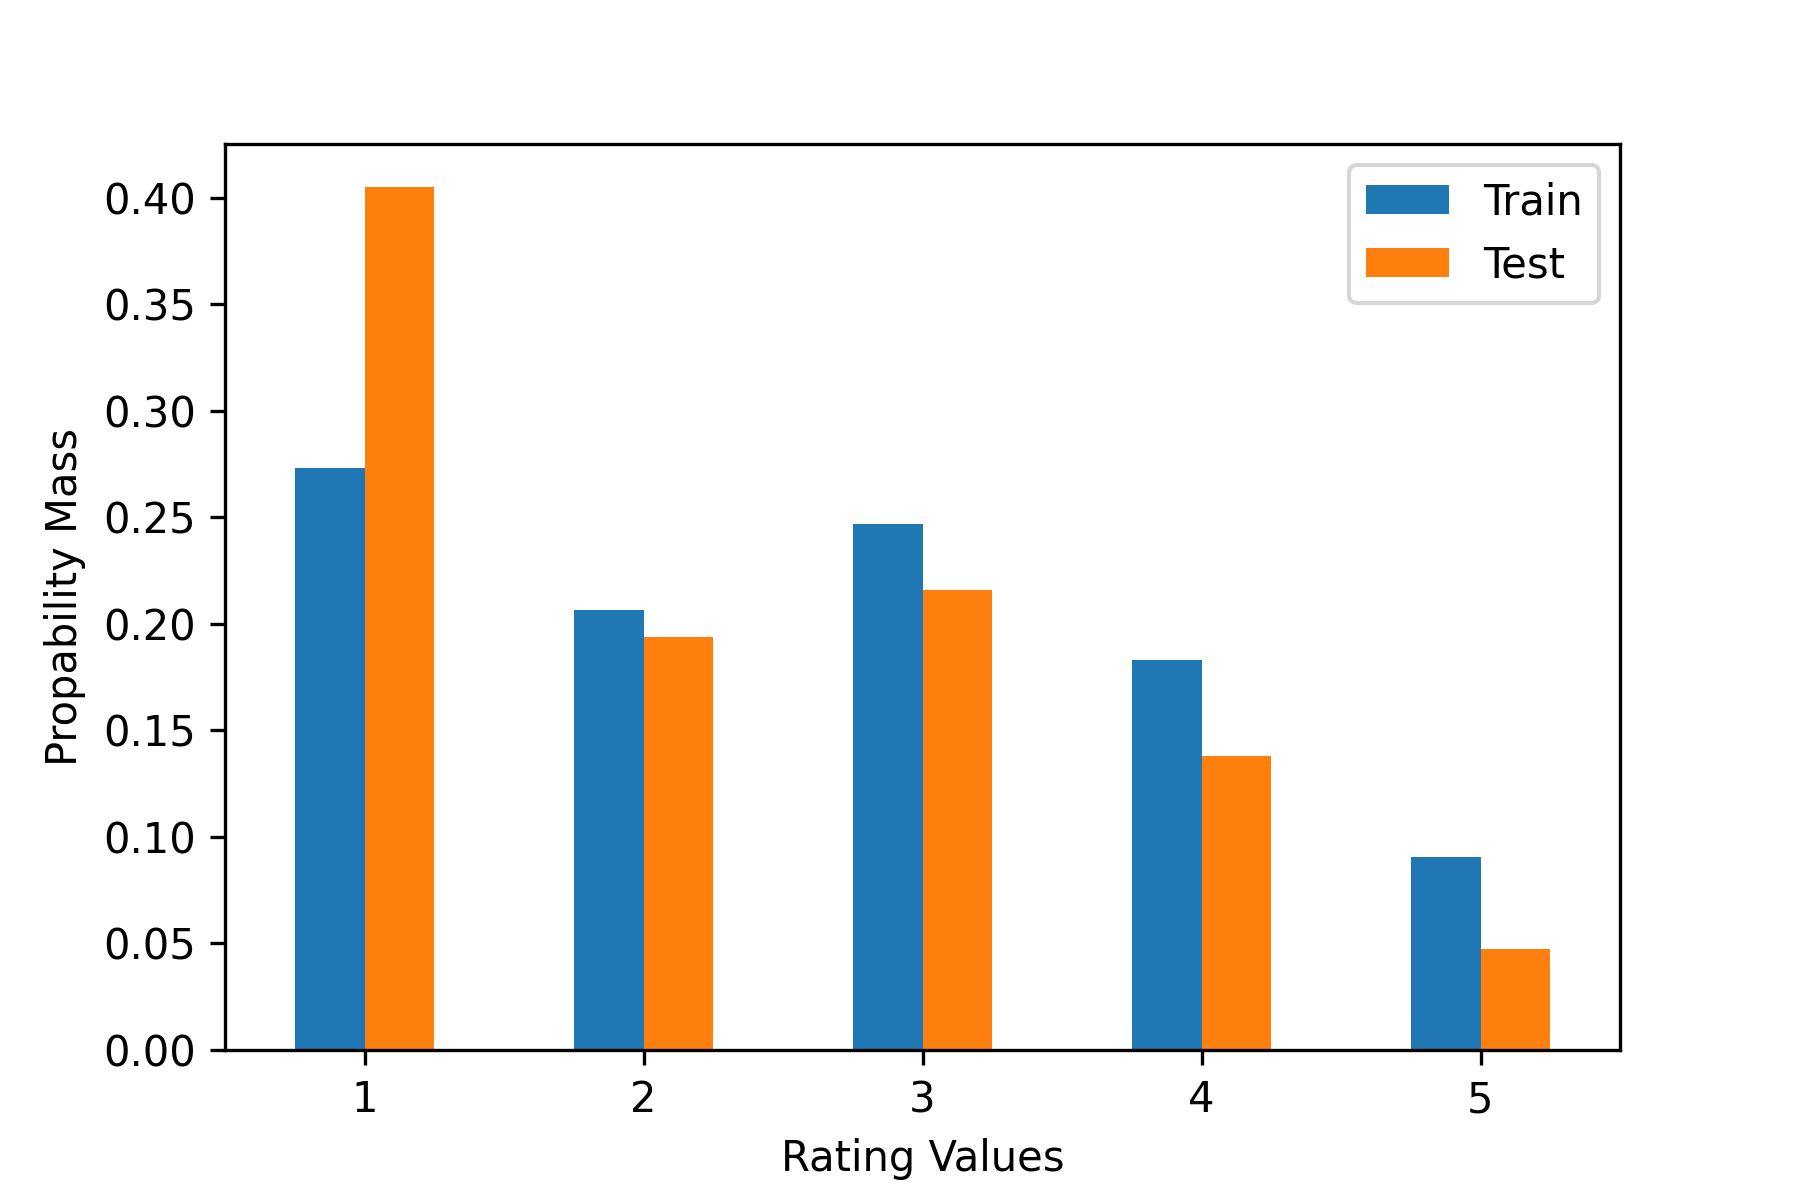
\includegraphics[width=\textwidth]{images/Chapter4/Diff_coat.png}
    \caption{So sánh phân phối xác suất các đánh giá trên tập huấn luyện bị lệch với tập kiểm tra không bị lệch của bộ dữ liệu Coat}
    \label{fig:4_1_coat}
\end{figure}

\begin{figure}[h]
    \centering
    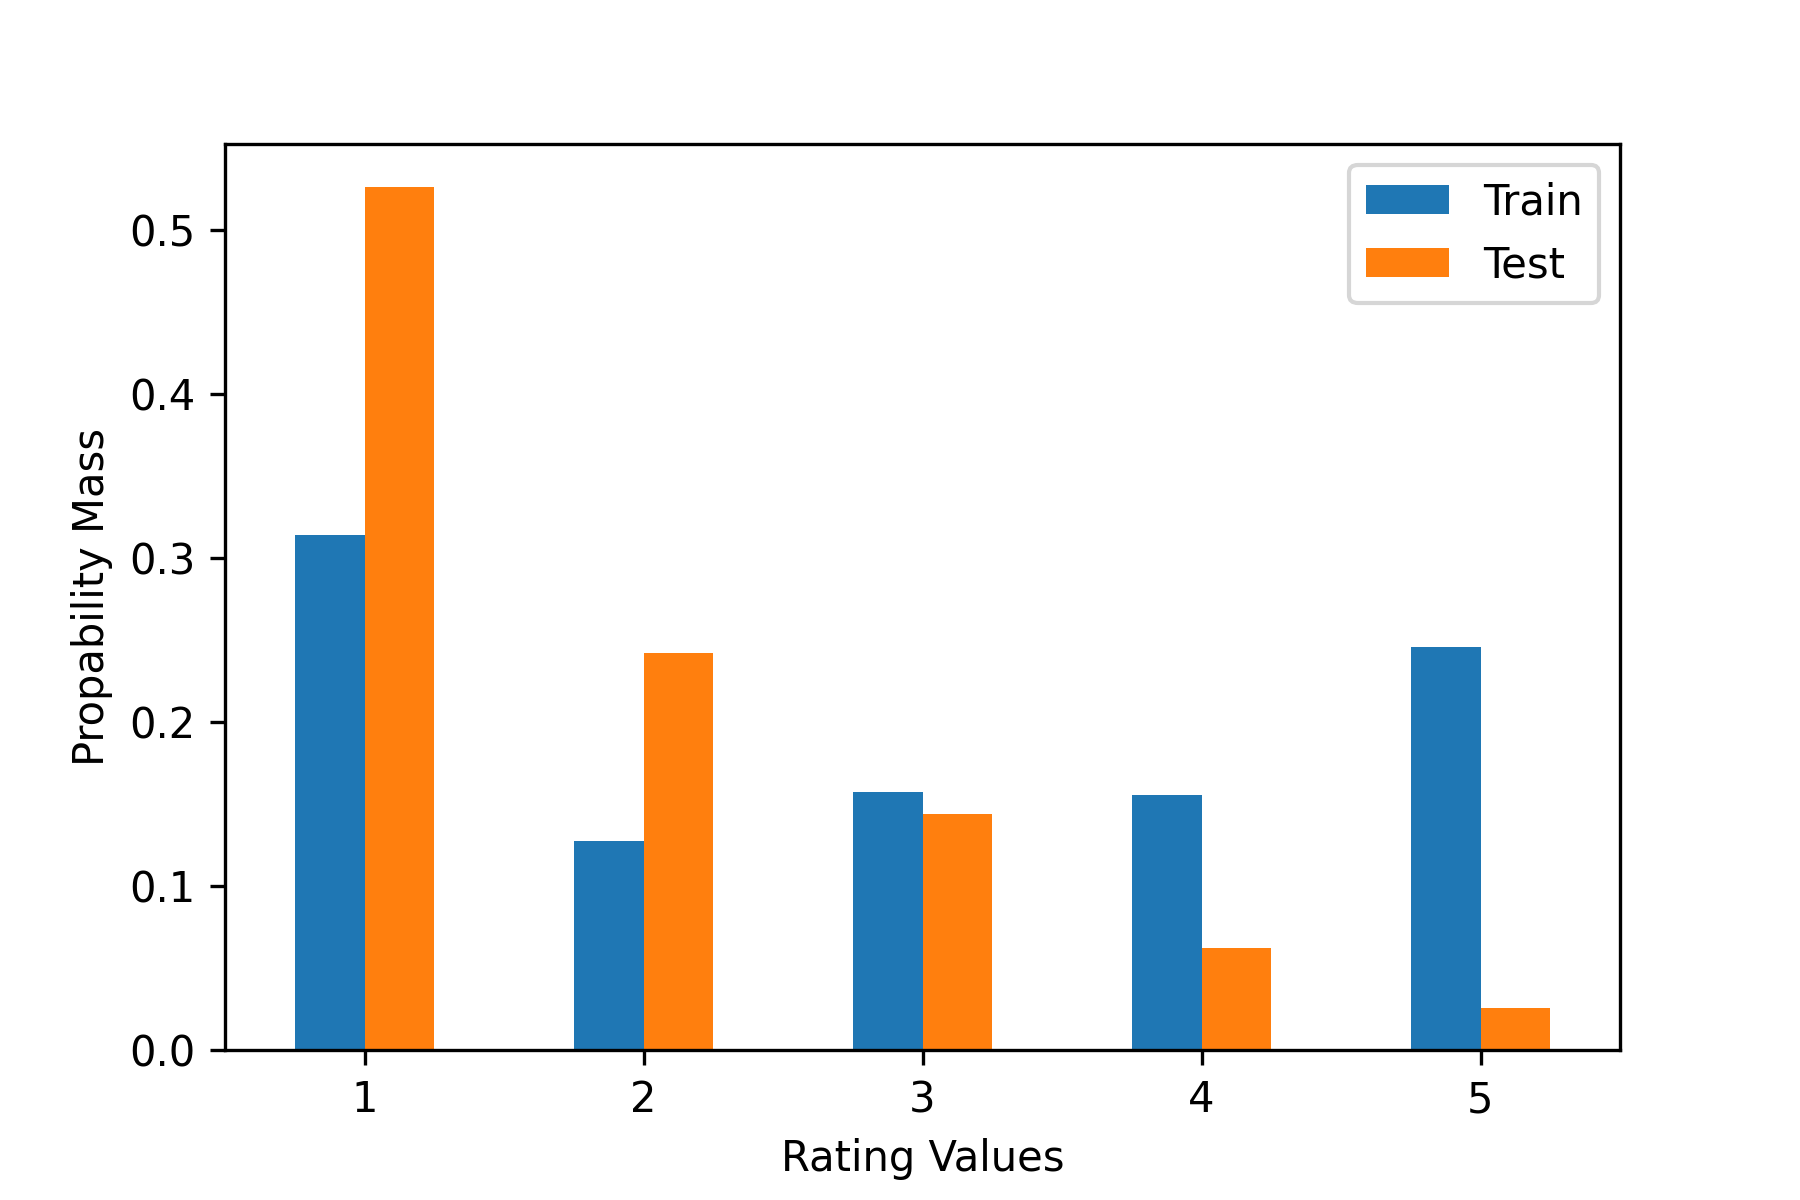
\includegraphics[width=\textwidth]{images/Chapter4/Diff_yahoo.png}
    \caption{So sánh phân phối xác suất các đánh giá trên tập huấn luyện bị lệch với tập kiểm tra không bị lệch của bộ dữ liệu Yahoo!R3}
    \label{fig:4_2_yahoo}
\end{figure}









\subsection{Mức độ cải thiện của MF-IPS với MF khi học trên tập MovieLens giả lập với mức độ thiên lệch của dữ liệu giảm dần}
\subsubsection{Tập MovieLens giả lập}
\label{subsubsection:MovieLens}
Như đã trình bày ở phần trước, ở thí nghiệm này nhóm chúng em sẽ tiến hành thí nghiệm trên tập dữ liệu MovieLens 100k. Vì thí nghiệm này yêu cầu kiểm soát được mức độ thiên lệch của dữ liệu, nên nhóm chúng em sẽ tiến hành tạo một tập dữ liệu MovieLens~100k giả lập. 

Tập dữ liệu MovieLens~100k giả lập sẽ được tạo bằng cách sử dụng mô hình MF được huấn luyện trên toàn bộ tập dữ liệu MovieLens 100k, để điền toàn bộ giá trị còn thiếu trong ma trận tương tác giữa người dùng và sản phẩm MovieLens~100k. Với [$p_1, p_2, p_3, p_4, p_5$] là phân bố của dữ liệu trong tập MovieLens~100k giả lập, $p_1$ là tỉ lệ đánh giá 1 trong toàn bộ dữ liệu và tương tự với các đánh giá còn lại, thì phân bố dữ liệu sau khi hoàn thành ma trận giả lập là [$0.001, 0.027, 0.601, 0.364, 0.007$]. Có thể thấy các đánh giá trong ma trận giả lập này bị lệch nghiêm trọng, với số lượng đánh giá 3 và 4 chiếm số lượng rất lớn khi so với các đánh giá 1, 2 và 5. Điều này rất vô lý trong thực tế, vì vậy nhóm chúng em tiến hành điều chỉnh lại ma trận giả lập này tuân theo phân bố dữ liệu của tập test trong tập Yahoo!R3 là [$0.526, 0.242, 0.144, 0.062, 0.026$].

Ngoài ra, dữ liệu quan sát được sẽ được ước lượng như sau: Với các đánh giá 4 và 5, propensity để quan sát được các đánh giá này $k$. Đối với các đánh giá < 4, propensity để quan sát được các đánh giá này là $k\alpha^{4-r}$, với $r$ là các đánh giá và $\alpha \in [0,1]$ là tham số điều chỉnh mức độ thiên lệch dữ liệu. Với mỗi $\alpha$. $k$ được đặt sao cho số lượng dữ liệu quan sát được chỉ chiếm 5\% trên toàn bộ ma trận. Bằng cách thay đổi giá trị $\alpha$, chúng ta có thể thay đổi được mức độ thiên lệch dữ liệu. Khi $\alpha = 1$ dữ liệu sẽ được phát sinh hoàn toàn ngẫu nhiên theo phân phối đều (vì khi đó propensity của toàn bộ đánh giá đều bằng $k$). Khi $\alpha \rightarrow 0$ thì dữ liệu quan sát được chỉ chứa các giá trị 4 và 5 (vì khi đó propensity của các đánh giá 1,2 và 3 bằng 0). Lưu ý là với $\alpha = 0.25$ thì phân bố của dữ liệu quan sát được sẽ giống với phân bố của dữ liệu MovieLens 100k ban đầu ([0.06, 0.11, 0.27, 0.35, 0.21] trong tập dữ liệu gốc và [0.06, 0.10, 0.25, 0.42, 0.17] trên tập dữ liệu quan sát được)

\subsubsection{Cách tiến hành}
Sau khi có bộ dữ liệu quan sát được ta sẽ tiến hành huấn luyện 2 mô hình MF và MF-IPS trên tập dữ liệu này. Hai mô hình này sẽ được cross-validation để chọn tham số $\lambda$ khác nhau và tham số $d$ sẽ được cố định với $d = 20$. Ta sẽ tiến hành thay đổi giá trị $\alpha$ từ [0.0625, 0.125, 0.25, 0.5, 1] để đo lường độ lỗi của hai mô hình MF và MF-IPS với mức độ thiên lệch của dữ liệu giảm dần.
\subsection{Kết quả}
Bảng \ref{table:4_movielens} mô tả kết quả thu được của nhóm em với độ lỗi MSE trên 2 mô hình MF và MF-IPS khi tiến hành thay đổi mức độ thiên lệch dữ liệu bằng cách thay đổi giá trị của $\alpha$. Có thể thấy khi mức độ thiên lệch của dữ liệu cao (khi $\alpha$ nhỏ) thì độ lỗi trên 2 mô hình MF và MF-IPS rất cao; đặc biệt, độ lỗi của mô hình MF-IPS mặc dù dữ liệu bị thiên lệch rất nhiều nhưng vẫn có độ lỗi thấp hơn đáng kể khi so sánh với mô hình MF. Khi giảm dần mức độ thiên lệch dữ liệu ($\alpha$ lớn) độ lỗi trên 2 mô hình này có sự cải thiện đáng kể và gần như xê xích nhau không nhiều, mặc dù vậy mô hình MF-IPS vẫn cho độ lỗi thấp hơn mô hình MF. 

\begin{table}[h]
    \centering
    \begin{tabular}{|c|c|c|}
    \hline
    alpha & MF & MF-IPS \\ \hline
    0.0625 & 1.701 & 1.199 \\ \hline
    0.125 & 0.706 & 0.444 \\ \hline
    0.25 & 0.221 & 0.164 \\ \hline
    0.5 & 0.114 & 0.102 \\ \hline
    1 & 0.112 & 0.109 \\ \hline
    \end{tabular}
    \caption{Độ lỗi MSE của hai mô hình MF và MF-IPS khi học trên tập MovieLens giả lập với mức độ thiên lệch của dữ liệu giảm dần.}
    \label{table:4_movielens}
\end{table}

Hình \ref{fig:4_movielens} minh họa rõ cho ta thấy sự cải thiện trong độ lỗi của 2 mô hình MF và MF-IPS thi mức độ thiên lệch của dữ liệu giảm dần.
\begin{figure}[h]
    \centering
    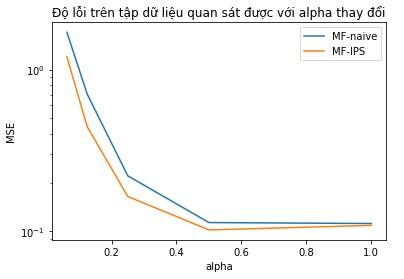
\includegraphics[width = \textwidth]{images/Chapter4/movielens.jpg}
    \caption{Hình ảnh minh họa sự cải thiện về độ lỗi của MF và MF-IPS khi thay đổi mức độ thiên lệch của dữ liệu}
    \label{fig:4_movielens}
\end{figure}

\section{Ảnh hưởng của việc ước lượng ma trận propensity tới việc học của MF-IPS}
Trong phần này, nhóm em sẽ thiết kế các thí nghiệm để làm rõ ảnh hưởng của việc ước lượng mà trận propensity đến việc học của MF-IPS. Việc ước lượng ma trận propensity có thể bị ảnh hưởng bởi hai yếu tố sau:
\begin{itemize}
    \item Phương pháp ước lượng sẽ ảnh hưởng đến hiệu quả của việc ước lượng. Do đó nhóm sẽ tiến hành ước lượng ma trận xu hướng bằng cả phương pháp Logistic Regression và phương pháp Naive Bayes trên cùng bộ dữ liệu Coat, vì chỉ bộ dữ liệu này mới chứa thông tin của người dùng và sản phẩm để có thể tiến hành ước lượng ma trận propensity bằng phương pháp Logistic Regression. 
\end{itemize}các cách ước lượng khác nhau, cụ thể là phương pháp ước lượng LL 

\subsection{So sánh mức độ cải thiện của MF-IPS với MF bằng các phương pháp ước lượng ma trận propensity khác nhau}


\subsection{So sánh mức độ cải thiện của MF-IPS với MF khi ước lượng ma trận propensity bằng Naive Bayes với số lượng dữ liệu MCAR khác nhau}



% \section{Đánh giá hiệu suất trên dữ liệu thế giới thực}
% \label{sec:4_performance}
% Mục tiêu: Nhằm đánh giá hiệu suất của mô hình ``Matrix factorization'' tiêu chuẩn (MF-Standard) và ``Matrix factorization'' (MF-IPS) sử dụng độ đo IPS trên 2 tập dữ liệu thế giới thực là Yahoo và Coat.

% Để sử dụng độ đo IPS trong việc huấn luyện mô hình ``Matrix Factorization'' trên 2 bộ dữ liệu ta tiến hành như sau:
% \begin{itemize}
%     \item Tập dữ liệu Yahoo: ta ước lượng ma trận xu hướng bằng phương pháp ``Naive Bayes''. Xác suất biên $P(Y=r)$ sẽ được tính toán thông qua 5\% của tập kiểm tra và 95\% còn lại sẽ được sử dụng để kiểm tra mô hình.
%     \item Tập dữ liệu Coat: ta ước lượng ma trận xu hướng bằng phương pháp ``Logistic Regression'' dựa trên hiệp biến của người dùng (giới tính, nhóm tuổi, vị trí và nhận thức về thời trang) và hiệp biến của sản phẩm (giới tính, loại áo khoác, màu sắc, và nó đã được khuyến mãi chưa). Mô hình ``Logistic Regression'' sẽ được huấn luyện bằng cách sử dụng tất cả các cặp hiệp biến của người dùng và sản phẩm làm các đặc trưng đầu vào, với nhãn là điểm đánh giá của người dùng cho các sản phẩm tương ứng; mô hình sẽ được cross-validation để tối ưu trên tập dữ liệu quan sát được do người dùng tự lựa chọn.
% \end{itemize}

% Kết quả: Bảng \ref{tab:4_performance} cho thấy hiệu suất của mô hình MF-IPS khi so sánh với MF-Standard, có thể thấy phương pháp MF-IPS có hiệu suất vượt trội hơn đáng kể khi so sánh với phương pháp thông thường.

% \begin{table}[h]
%     \centering
%     \begin{tabular}{|l|ll|ll|}
%     \hline
%     \multirow{2}{*}{} & \multicolumn{2}{c|}{Yahoo} & \multicolumn{2}{c|}{Coat} \\ \cline{2-5} 
%      & \multicolumn{1}{l|}{MAE} & MSE & \multicolumn{1}{l|}{MAE} & MSE \\ \hline
%     MF-IPS & \multicolumn{1}{l|}{0.810} & 0.989 & \multicolumn{1}{l|}{0.860} & 1.093 \\ \hline
%     MF-Standard & \multicolumn{1}{l|}{1.154} & 1.891 & \multicolumn{1}{l|}{0.920} & 1.202 \\ \hline
%     \end{tabular}
%     \caption{Hiệu suất trên 2 tập dữ liệu Yahoo và Coat}
%     \label{tab:4_performance}
% \end{table}

% \section{Dữ liệu thiên lệch ảnh hưởng đến việc đánh giá như thế nào?}
% \label{sec:4_evaluate}



% \section{Dữ liệu thiên lệch ảnh hưởng đến việc học như thế nào?}
% \label{sec:4_learning}
% \section{Tính mạnh mẽ của điểm xu hướng đã học không chính xác trong việc học và đánh giá mô hình như thế nào?}
% \label{sec:4_robust}

